% =============================================================================
% sections/design/drone/physical_design/airframe_landing_platform.tex  -  Airframe and Landing Platform
% Teams: drone (best guess - unconfirmed) / Status: EXAMPLE (scope approximation)
%
% EXAMPLE CONTENT for scope/layout approximation - not final report text.
% Scope covers the physical airframe, custom 3D-printed parts, electronics
% enclosures, custom mounting brackets, and the design and integration of the
% rover-mounted landing platform. Marked with \exampleflag on its heading in
% the assembler.
% =============================================================================

\begin{figure}[!htbp]
    \centering
    \begin{subfigure}[b]{0.3\textwidth}
        \centering
        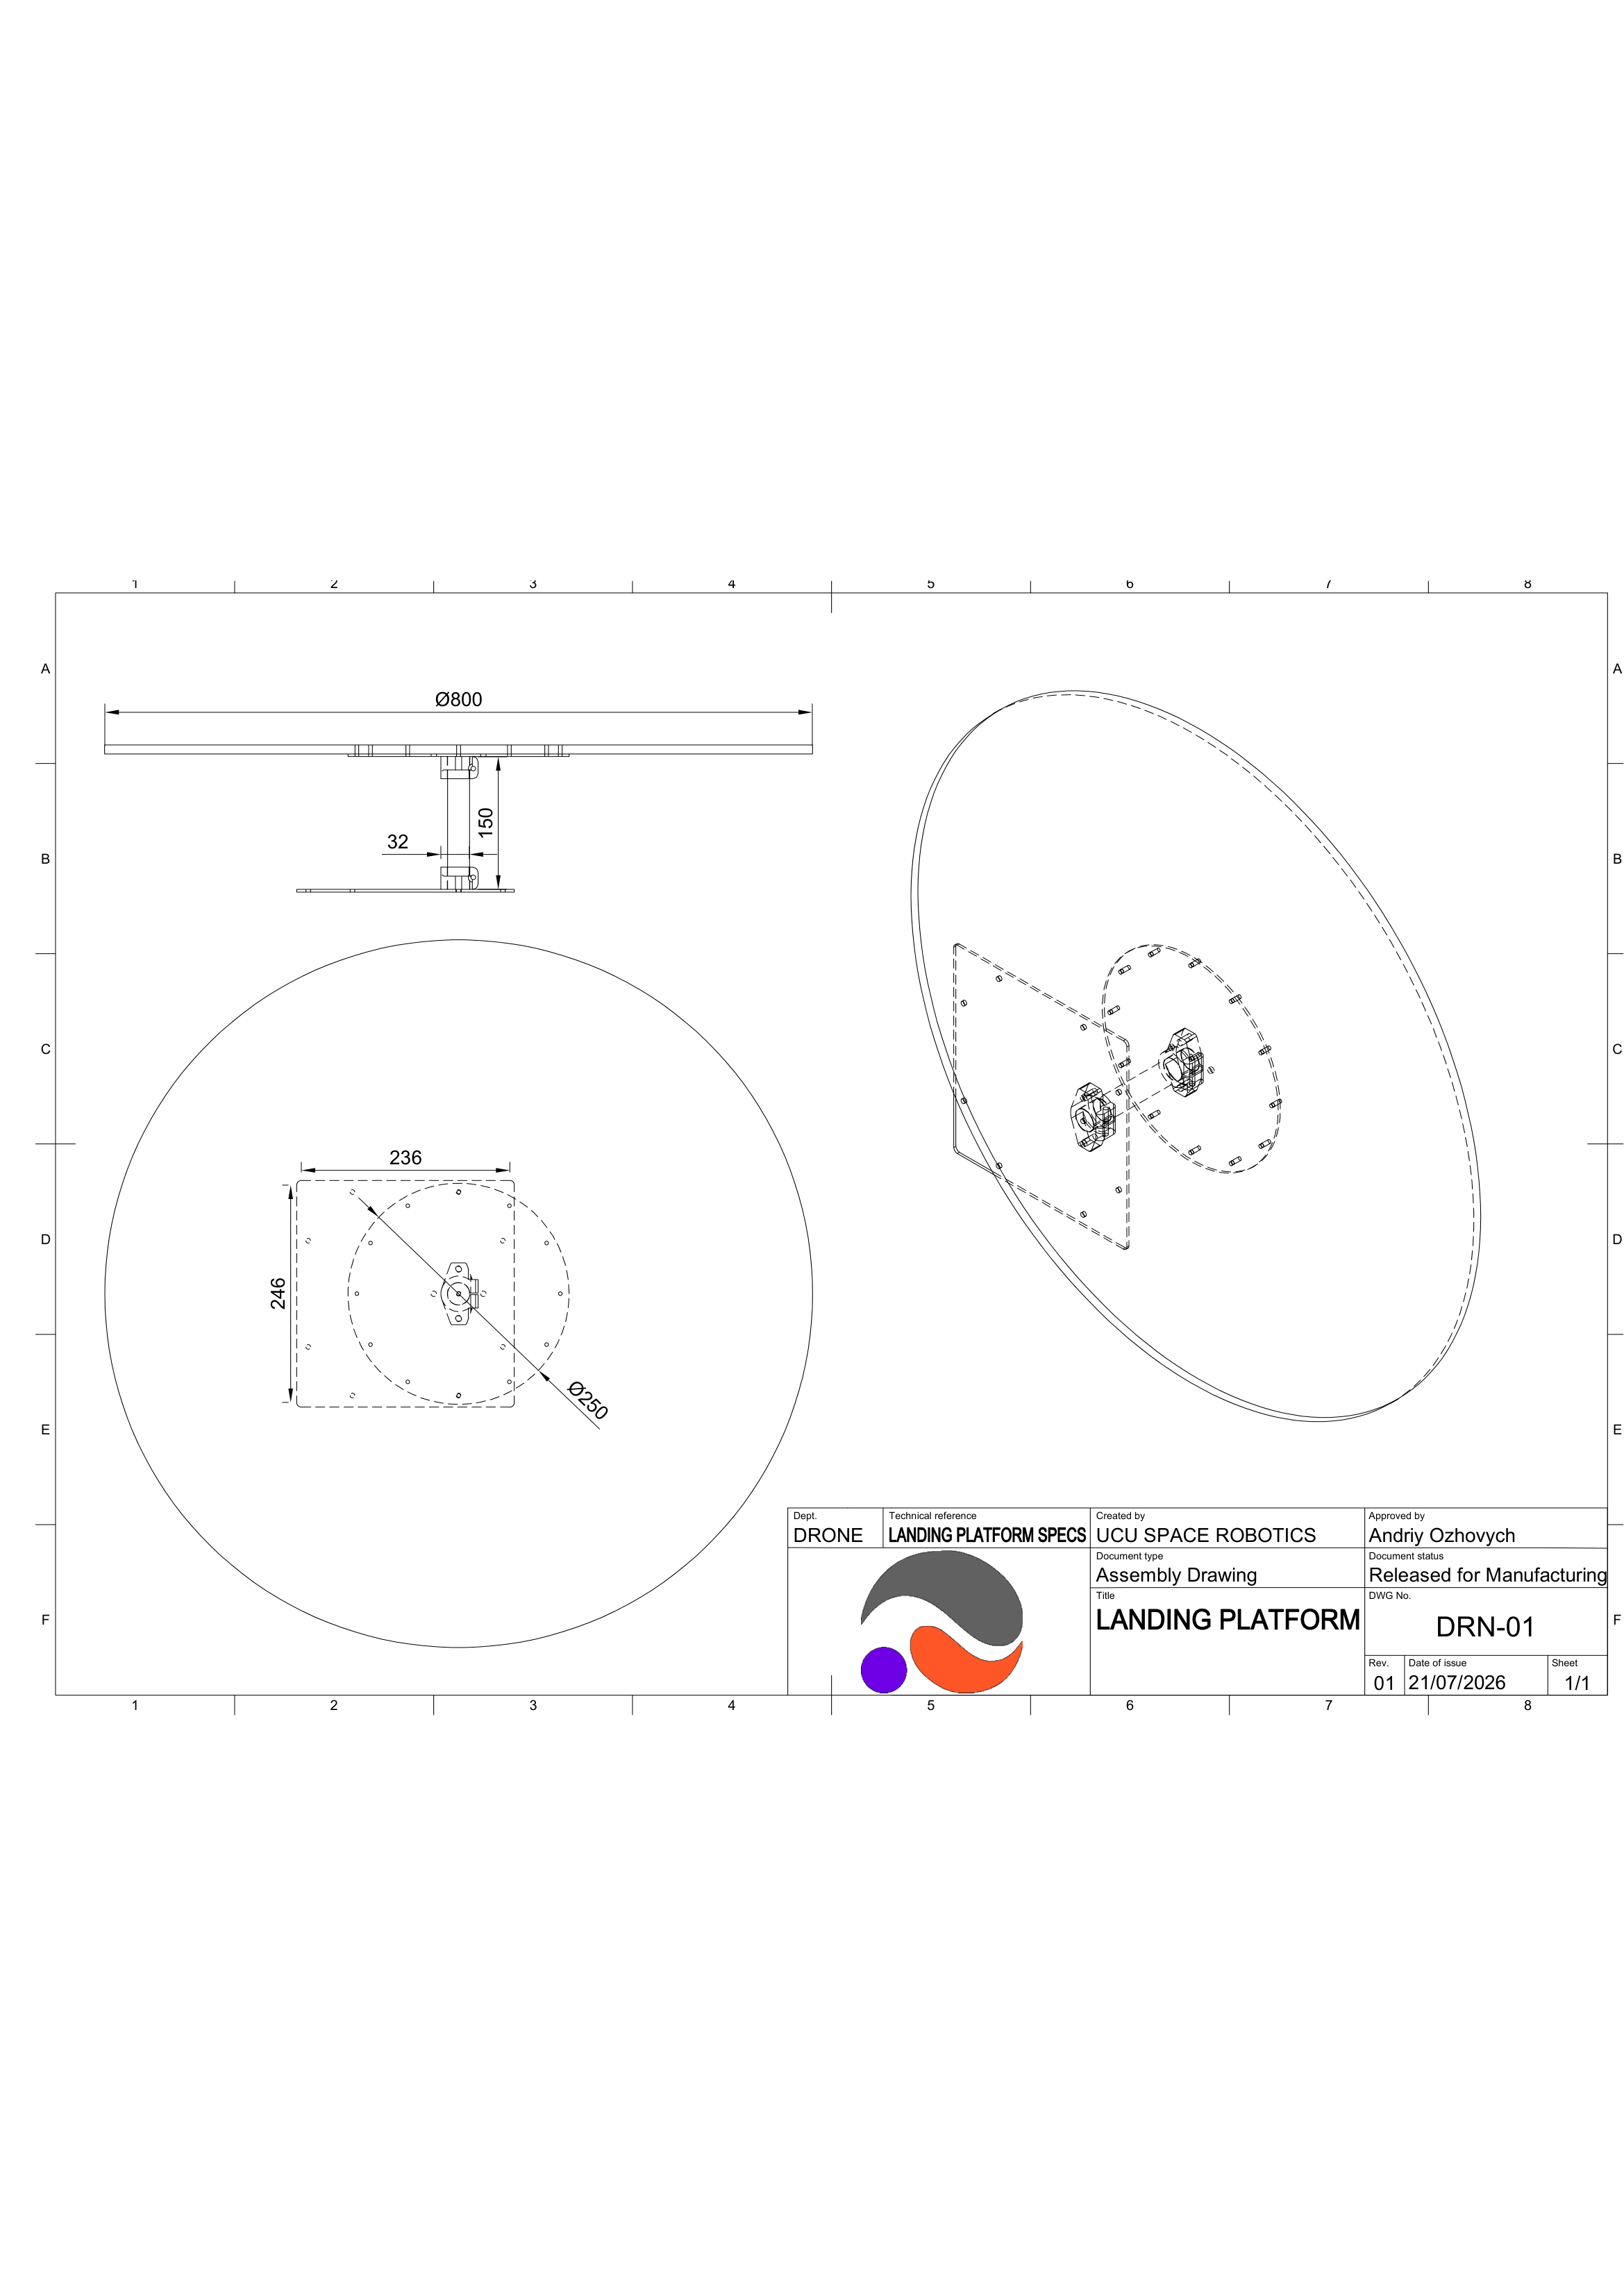
\includegraphics[width=\linewidth]{teams/drone/figures/drone_landing_platform_blueprint.png}
        \caption{Landing platform drawing}
    \end{subfigure}
    \hfill
    \begin{subfigure}[b]{0.48\textwidth}
        \centering
        
\includegraphics[width=\linewidth]{teams/suspension/figures/rocker_suspension_obstacle}
        \caption{Manufactured landing platform}
    \end{subfigure}
    \caption{Platform}\label{fig:platform}
\end{figure}

To perform the additional task within the Droning Sub-Task, 
the rover is equipped with a modular landing platform with 
a radius of \qty{0.4}{\meter}. The platform consists of a 
plywood landing surface reinforced by a steel support disc 
to provide the required structural stiffness during autonomous 
take-off and landing. It is mounted on the upper chassis and 
can be rapidly installed or removed. \autoref{fig:platform}

\todo[inline]{Add a dimensioned drawing or photo of the landing platform
mounted on the rover - the Preliminary described it in prose only.}

